\documentclass[conference]{IEEEtran}

\usepackage{cite}
\usepackage{amsmath}
\usepackage{amssymb}
\usepackage{url}
\usepackage{graphicx}
\usepackage{booktabs}
\usepackage{microtype}
\usepackage[table]{xcolor}
\usepackage{tikz}
\usetikzlibrary{positioning,arrows.meta,fit,backgrounds}
\usepackage{pgfplots}
\pgfplotsset{compat=1.18}
\usepgfplotslibrary{groupplots}
\usepackage[hidelinks]{hyperref}

\definecolor{phaseblue}{RGB}{52,152,219}
\definecolor{phasegreen}{RGB}{46,204,113}
\definecolor{phaseorange}{RGB}{230,126,34}
\definecolor{phasepurple}{RGB}{155,89,182}
\definecolor{phase1blue}{RGB}{52,152,219}
\definecolor{phase2green}{RGB}{46,204,113}
\definecolor{phase3orange}{RGB}{230,126,34}
\definecolor{phase4purple}{RGB}{155,89,182}
\definecolor{softgray}{RGB}{245,247,250}

\title{{\LARGE\textbf{Fairness-Aware Bandits for Network Routing in Quantum \& Clinical Settings}}\\
{\Large\textit{via Multi-Armed, Contextual, and Informative Contextual Decision Spectra}}}

\author{
\IEEEauthorblockN{Piter Z. Garcia}
\IEEEauthorblockA{MS Data Science / Decision-Making \& Algorithmic Fairness\\
Rochester Institute of Technology (RIT)\\
pizg8794@g.rit.edu}
\and
\IEEEauthorblockN{Daniel Krutz, Travis Desell}
\IEEEauthorblockA{Department of Software Engineering, Data Science\\
Rochester Institute of Technology (RIT)\\
dxkvse@g.rit.edu, tjdvse@g.rit.edu}
}

\begin{document}
\maketitle

\begin{abstract}
Sequential decision systems increasingly determine how scarce diagnostic,
computational, and communication resources are routed under uncertainty. This
study examines fairness-aware bandits across a decision spectrum, from
non-contextual multi-armed bandits to contextual and informative contextual
bandits, for settings where context is missing, delayed, noisy, or
group-dependent. The central claim is that quantum routing and clinical
diagnostic routing share a common sequential resource-allocation structure:
policies must choose actions from partial feedback, yet groups or flows with
the least reliable context can absorb the worst errors.

The work develops a reusable evaluation framework for this bandit spectrum
across two executable environment families. The quantum domain builds on a
state-preserving quantum-routing evaluation stack, while the clinical domain
uses an embedded synthetic clinical environment with resource allocation,
clinical models, and EQUITAS-mediated fairness reporting. Preliminary quantum
results show that predictive-context policies improve over no-context
baselines by 3.74 percentage points internally and 2.83 percentage points
externally. In the clinical setting, the embedded EQUITAS-aware allocator
improves oracle-normalized efficiency from 75.09\% to 91.23\%, raises mean
success from 50.0\% to 72.5\%, and reduces the latency parity gap from 18.0
to 10.17 relative to the baseline. In the related bioinformatics proxy,
context-aware scoring increases predicted-pair output from
14.96 $\pm$ 10.45 to 61.36 $\pm$ 44.21, with optimized output reaching
66.07 $\pm$ 46.36 and average disparate-impact improvement of +0.805 after
augmentation. Together, these components define a method for measuring and
mitigating time-evolving fairness disparities while preserving utility under
non-stationarity and limited context.
\end{abstract}

\begin{IEEEkeywords}
Fairness-aware bandits, contextual bandits, resource allocation, clinical
routing, quantum routing, partial feedback, missing context, algorithmic
fairness.
\end{IEEEkeywords}

\section{Introduction}

Many applied data science systems are sequential decision systems that route
limited resources under uncertainty: which diagnostic test to order, which case
to escalate, which model or pipeline to trust, or which quantum-network path
should receive scarce entanglement-generation attempts. These decisions are
difficult because the system observes only partial feedback. The chosen action
reveals an outcome, but the unchosen alternatives remain counterfactual. They
are also fairness critical because the quality of observed context is often
uneven across clinical groups, sites, and cohorts or across quantum flows and
service classes. When one population has delayed testing, incomplete patient
history, lower-quality measurements, or less representative calibration data,
a policy optimized only for aggregate reward can hide subgroup errors and
compound disparities over time. The same structure appears in quantum routing
when flows depend on uneven link, fidelity, capacity, or route-state evidence.

\begin{figure}[!t]
\centering
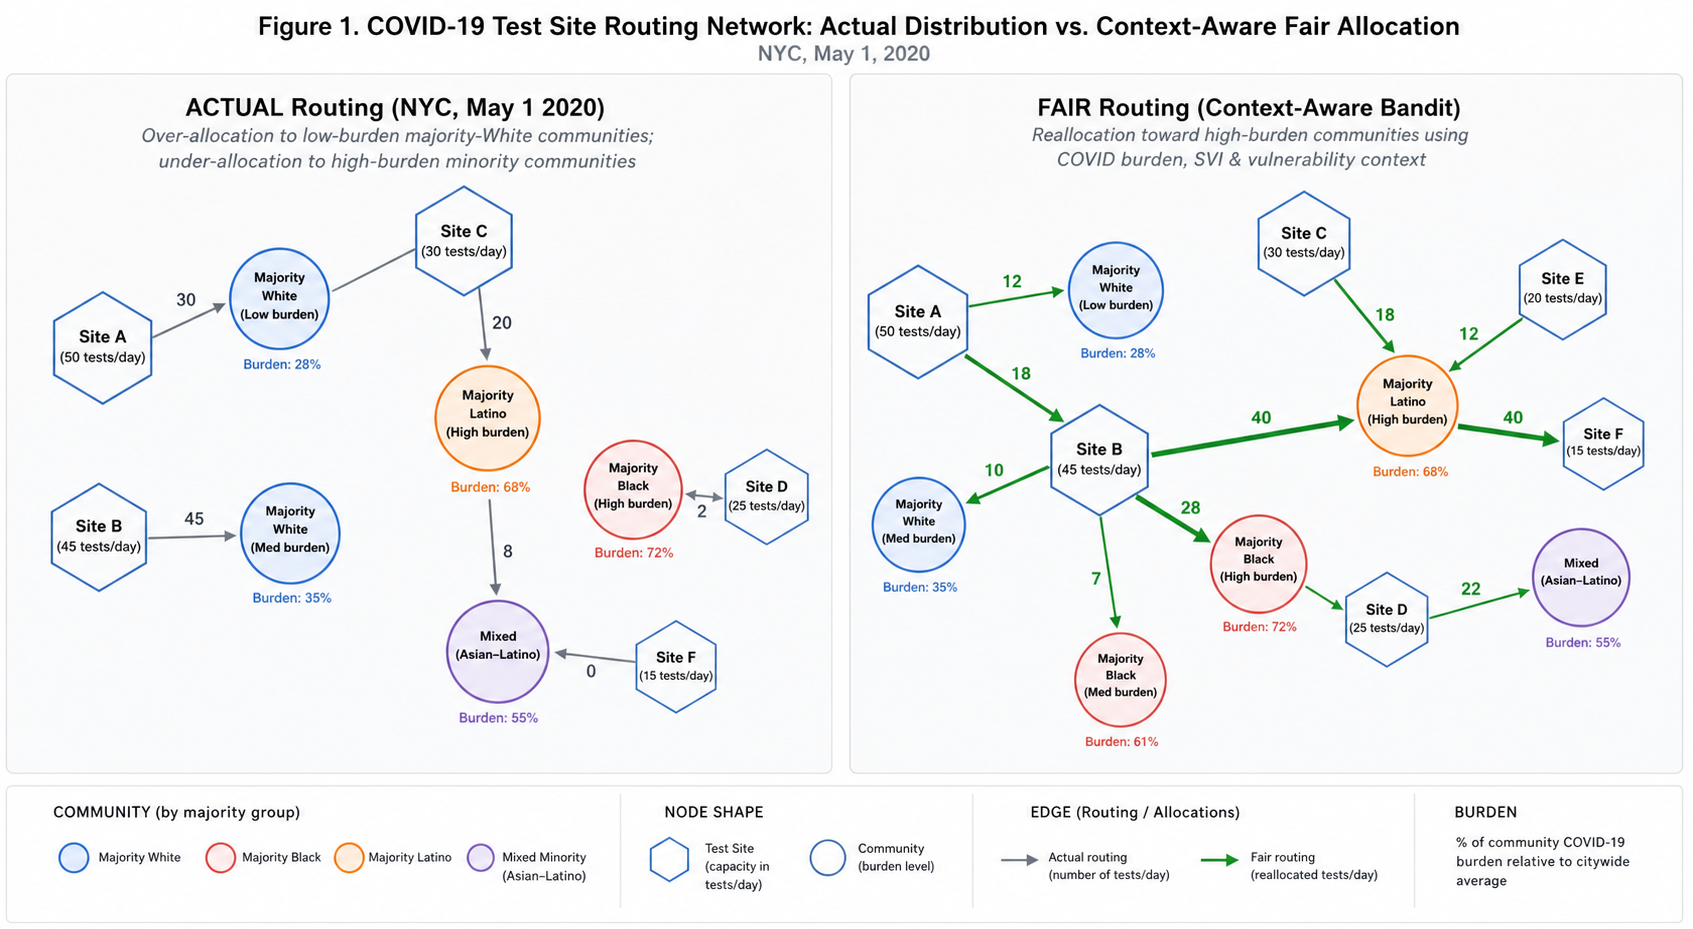
\includegraphics[width=0.98\columnwidth]{figures/clinical_routing_context_comparison.png}
\vspace{0.25em}
\caption{Real-world clinical routing illustration. The left side shows
weak-context allocation, while the right side shows context-aware fairness
allocation under the same shared routing problem.}
\label{fig:intro_clinical_routing}
\end{figure}

Figure~\ref{fig:intro_clinical_routing} summarizes this shared routing pattern
in the clinical domain; Appendix~\ref{app:quantum_routing_example} provides
the analogous quantum-routing example.

This work frames the scarce-resource routing problem as fairness-aware bandit
learning across a decision spectrum. At each round, a policy observes available
context, chooses an action, receives reward only for the chosen action, and
updates its future decisions. The scientific questions focus on whether
movement along the bandit spectrum reduces disparities when context is
missing, delayed, noisy, or group-dependent. This matters in clinical workflows
because false-negative, delayed-escalation, or under-testing gaps can produce
direct harm. It also matters in quantum-network routing because future
communication systems will allocate scarce probabilistic resources among
competing flows; fairness in success probability and latency is a
service-quality requirement.

The study develops a shared environment--runner--evaluator architecture for
two complementary routing domains. The first is a quantum-routing testbed
based on hybrid contextual bandits for entanglement routing and qubit
allocation~\cite{garcia2026threat_aware_quantum_routing}. It exposes noisy
links, uncertain entanglement generation, adversarial or non-stationary
conditions, allocator decisions, and saved evaluator state. The second is an
embedded clinical simulation motivated by equitable bioinformatics and
fairness auditing work~\cite{garcia2025equitable_bioinformatics}. It models
test ordering, retesting, escalation, diagnostic attention, model-assisted
triage, site-level constraints, and cohort-level context quality. The shared
abstraction is that each domain routes scarce resources under partial feedback
while fairness risk emerges from unequal context quality.

Four scientific research questions drive this work. RQ1 asks how much quality
context improves utility and fairness relative to non-contextual baselines.
RQ2 asks how quickly disparities emerge when a group, site, cohort, or flow
class receives noisier, delayed, or incomplete context. RQ3 asks whether
fairness-mediated policy updates reduce outcome gaps without unacceptable
utility loss. RQ4 asks whether the same fairness mediation strategy transfers
between clinical diagnostic simulation and quantum routing, or whether
mitigation must remain domain-specific. Our preliminary evidence supports the
context-gain premise: predictive-context quantum policies improve over
no-context baselines by 3.74 percentage points internally and 2.83 percentage
points externally. In the embedded clinical setting, the EQUITAS-aware
allocator improves oracle-normalized efficiency from 75.09\% to 91.23\%,
raises mean success from 50.0\% to 72.5\%, and reduces the latency parity gap
from 18.0 to 10.17 relative to the baseline.

\appendices
\section{Quantum Routing Motivating Example}
\label{app:quantum_routing_example}

\begin{figure}[!t]
\centering
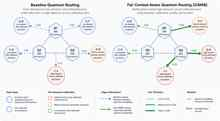
\includegraphics[width=0.98\columnwidth]{figures/quantum_routing_context_comparison.png}
\vspace{0.25em}
\caption{Quantum routing example corresponding to the clinical routing pattern
shown in Figure~\ref{fig:intro_clinical_routing}. The left side shows baseline
routing and the right side shows context-aware fairness allocation, illustrating
how the same partial-feedback and context-quality issue appears in quantum
network routing.}
\label{fig:appendix_quantum_routing}
\end{figure}

\bibliographystyle{IEEEtran}
\bibliography{rough_draft_references}

\end{document}
